\chapter{Проблемы обучения глубоких нейронных сетей}

В данной главе вводится теоретическая основа для понимания основных концепций теории обучения глубоких нейронных сетей. Приводится классификация основных типов слоев и архитектур моделей. Описывается историческая ретроспектива развития теории обучения глубоких моделей, а также основные проблемы, которые возникали и возникают при выполнении обучения. 

Осуществляется обзор существующих подходов для обучения глубоких нейронных сетей. Приводится описание методов обучения с использованием стохастического градиентого спуска и функций активации ReLU с ее вариантами. Описываются основные проблемы, присущие подобному типу обучения.

Особое внимание уделяется методам неконтролируемого предобучения, для реализации которых не требуется наличие объемной обучающей выборки. При выполнении предобучения осуществляется начальная инициализация параметров глубокой нейронной сети. Подобная инициализация позволяет уменьшить величину ошибки на этапе дообучения (<<тонкой настройки>>) и гарантирует его сходимость.

Приводятся алгоритмы предобучения с использованием RBM и автоэнкодерных моделей, формируемых из слоев ГНC и описывается этап <<тонкой настройки>> нейронной сети, цель которого состоит в дообучении модели для решения определенной задачи.

\section{Общие сведения}

Вопросы разработки и применения нейросетевых моделей часто рассматриваются в контексте более широкой области машинного обучения, являющейся по сути одним из направлений современной науки об искусственном интеллекте. При этом само машинное обучение сформировалось на стыке нескольких научных дисциплин, включающих вычислительную математику, теорию вероятностей и статистику, линейную алгебру и теорию оптимизации. С помощью алгоритмов машинного обучения создаются модели, которые используют предшествующий опыт для повышения эффективности компьютера в решении определенных классов задач \cite[c.~2]{mitchell1997machine}. Под понятием предшествующего опыта здесь понимается совокупность статистических данных, собранных при наблюдении и описании некоторого процесса. 

Являясь моделями машинного обучения, нейронные сети также способны к решению различных типов задач после реализации итеративного алгоритма настройки параметров, называемого обучением. Само свойство обучаемости приближает искусственные нейросети к их естественному прототипу, а именно к человеческому мозгу, обучение которого является важным процессом и формирует индивидуальность \cite[с.~316-317]{kandel}.

В основе теории искусственных нейронных сетей лежит биологически инспирированная модель искусственного нейрона, представляющая собой вычислительный элемент, выполняющий преобразование входных данных (рисунок \ref{fig:pic0_1}). Данное преобразование заключается в вычислении некоторой функции активации (линейной или нелинейной) $F$ от взвешенной суммы $S$ компонент вектора входных данных $X = (x_1, x_2, ..., x_n)$. Параметры $W = (w_1, w_2, ..., w_n)$ называются весовыми коэффициентами (весами) нейрона и настраиваются в процессе обучения в соответствии с определенным правилом обучения. Помимо весовых коэффициентов, у нейрона может быть дополнительный параметр $T$, называемый порогом (или пороговым коэффициентом). Он определяет смещение взвешенной суммы $S$.

\begin{figure}[H]
  \centering
  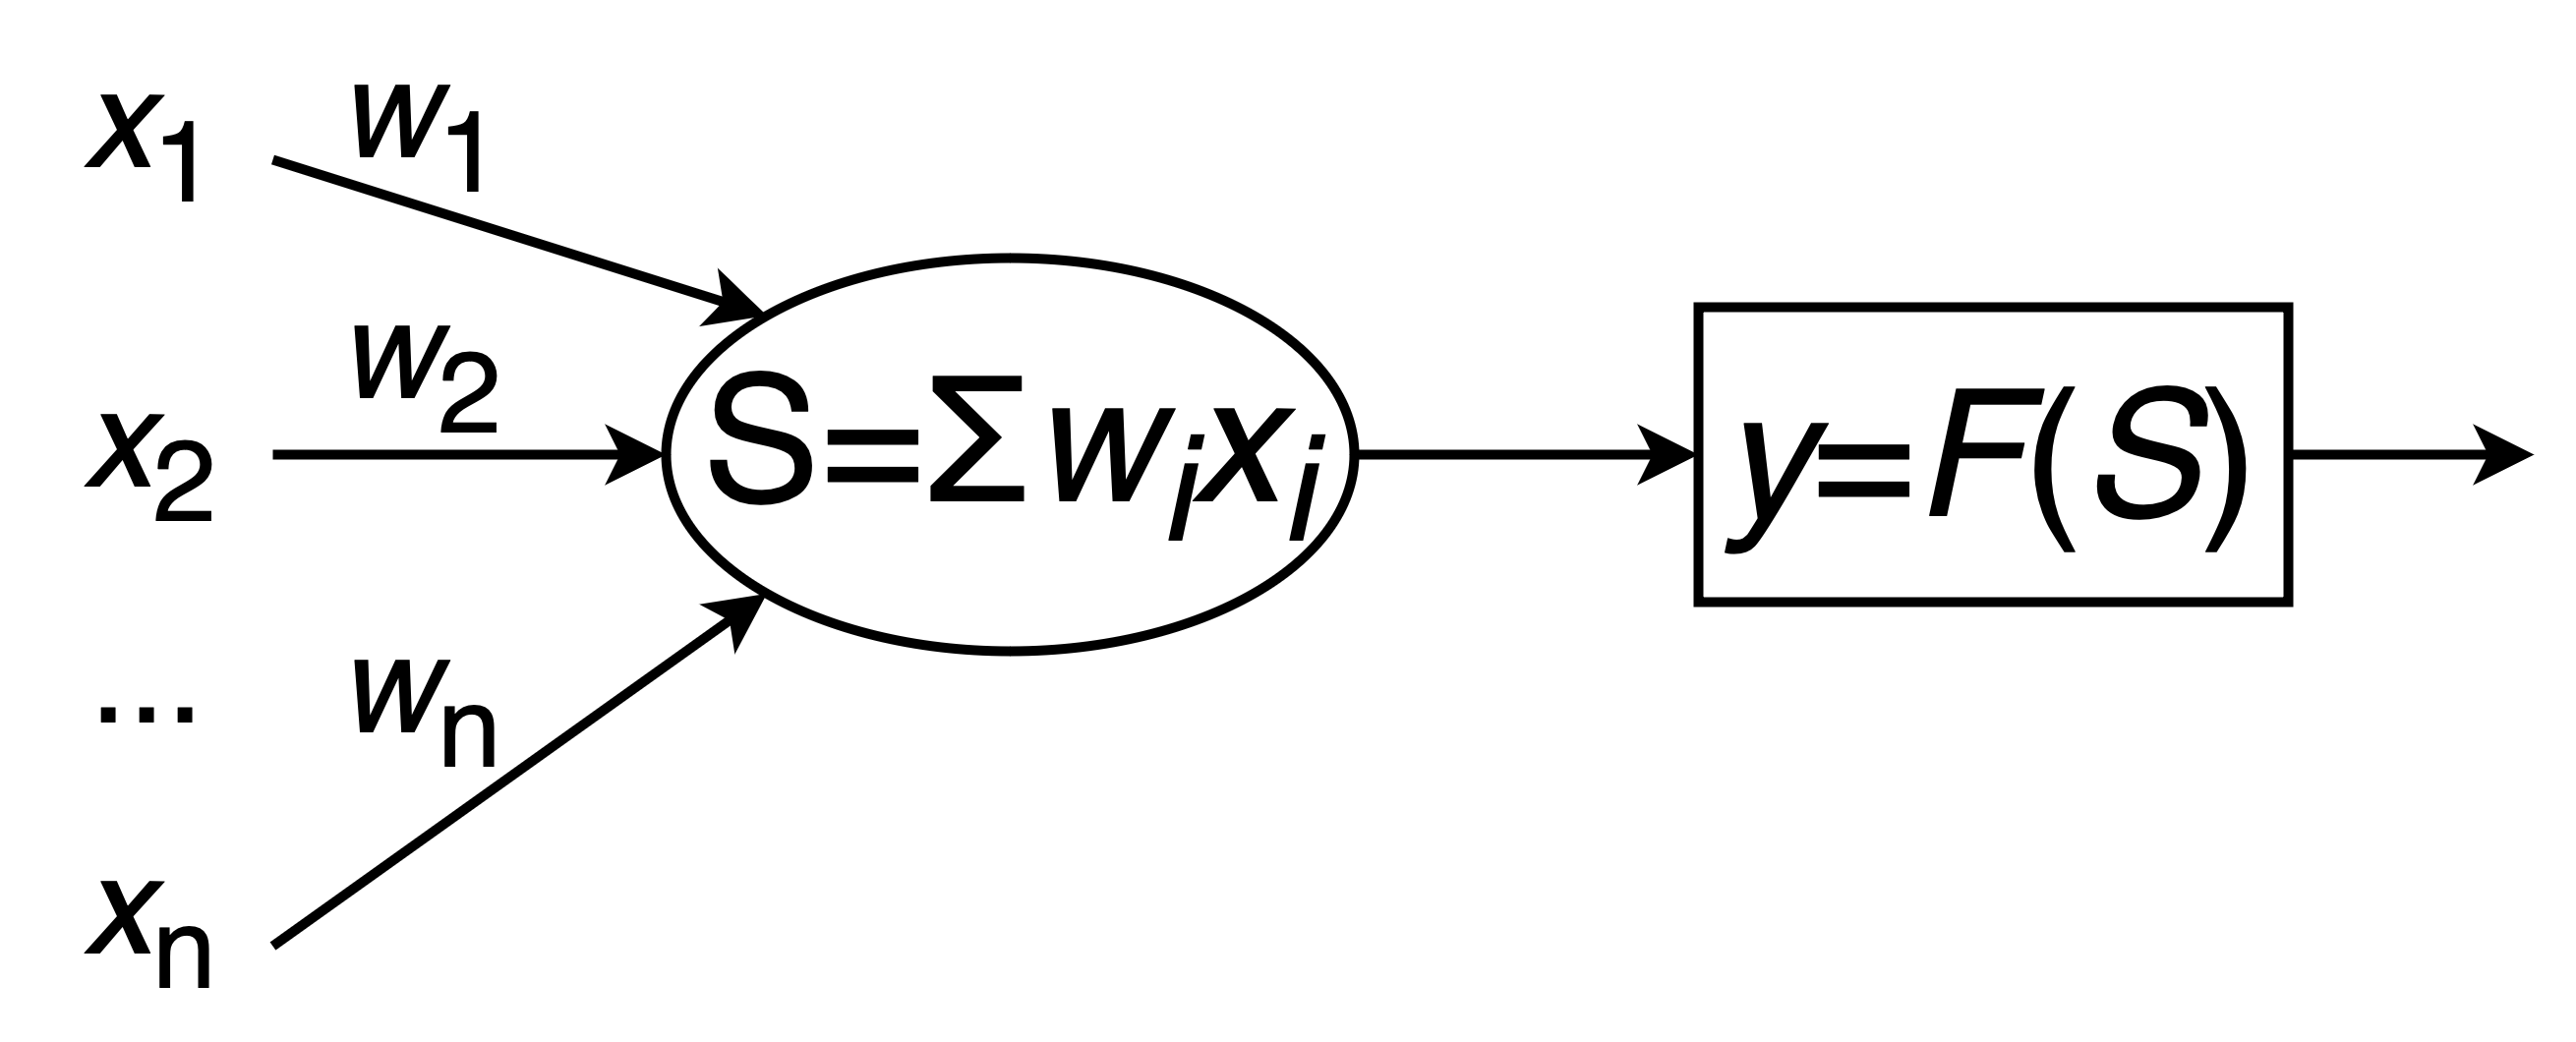
\includegraphics[width=\textwidth]{man-source/images/ch1/pic0-1.png}
  \caption{Модель искусственного нейрона}
  \label{fig:pic0_1}
\end{figure}

Искусственные нейроны могут быть объединены в группы, называемые слоями, по аналогии с биологическими нейронными слоями. Каждый нейрон слоя, обладая независимым набором весовых коэффициентов, получает на вход одинаковый вектор данных $X$ и выполняет его преобразование, формируя отдельную компоненту выходного вектора $Y$, называемого паттерном выходной активности слоя \cite[c.~27]{golovko2017} (рисунок \ref{fig:pic0_2}). Весовые коэффициенты отдельных нейронов для удобства объединяются в матрицу, которая называется матрицей весовых коэффициентов слоя (или матрицей весов). Слой, имеющий настраиваемые параметры, называется обрабатывающим (в отличие от распределительных слоев, которые являются предваряющими в любой НС и не имеют параметров).

\begin{figure}[H]
  \centering
  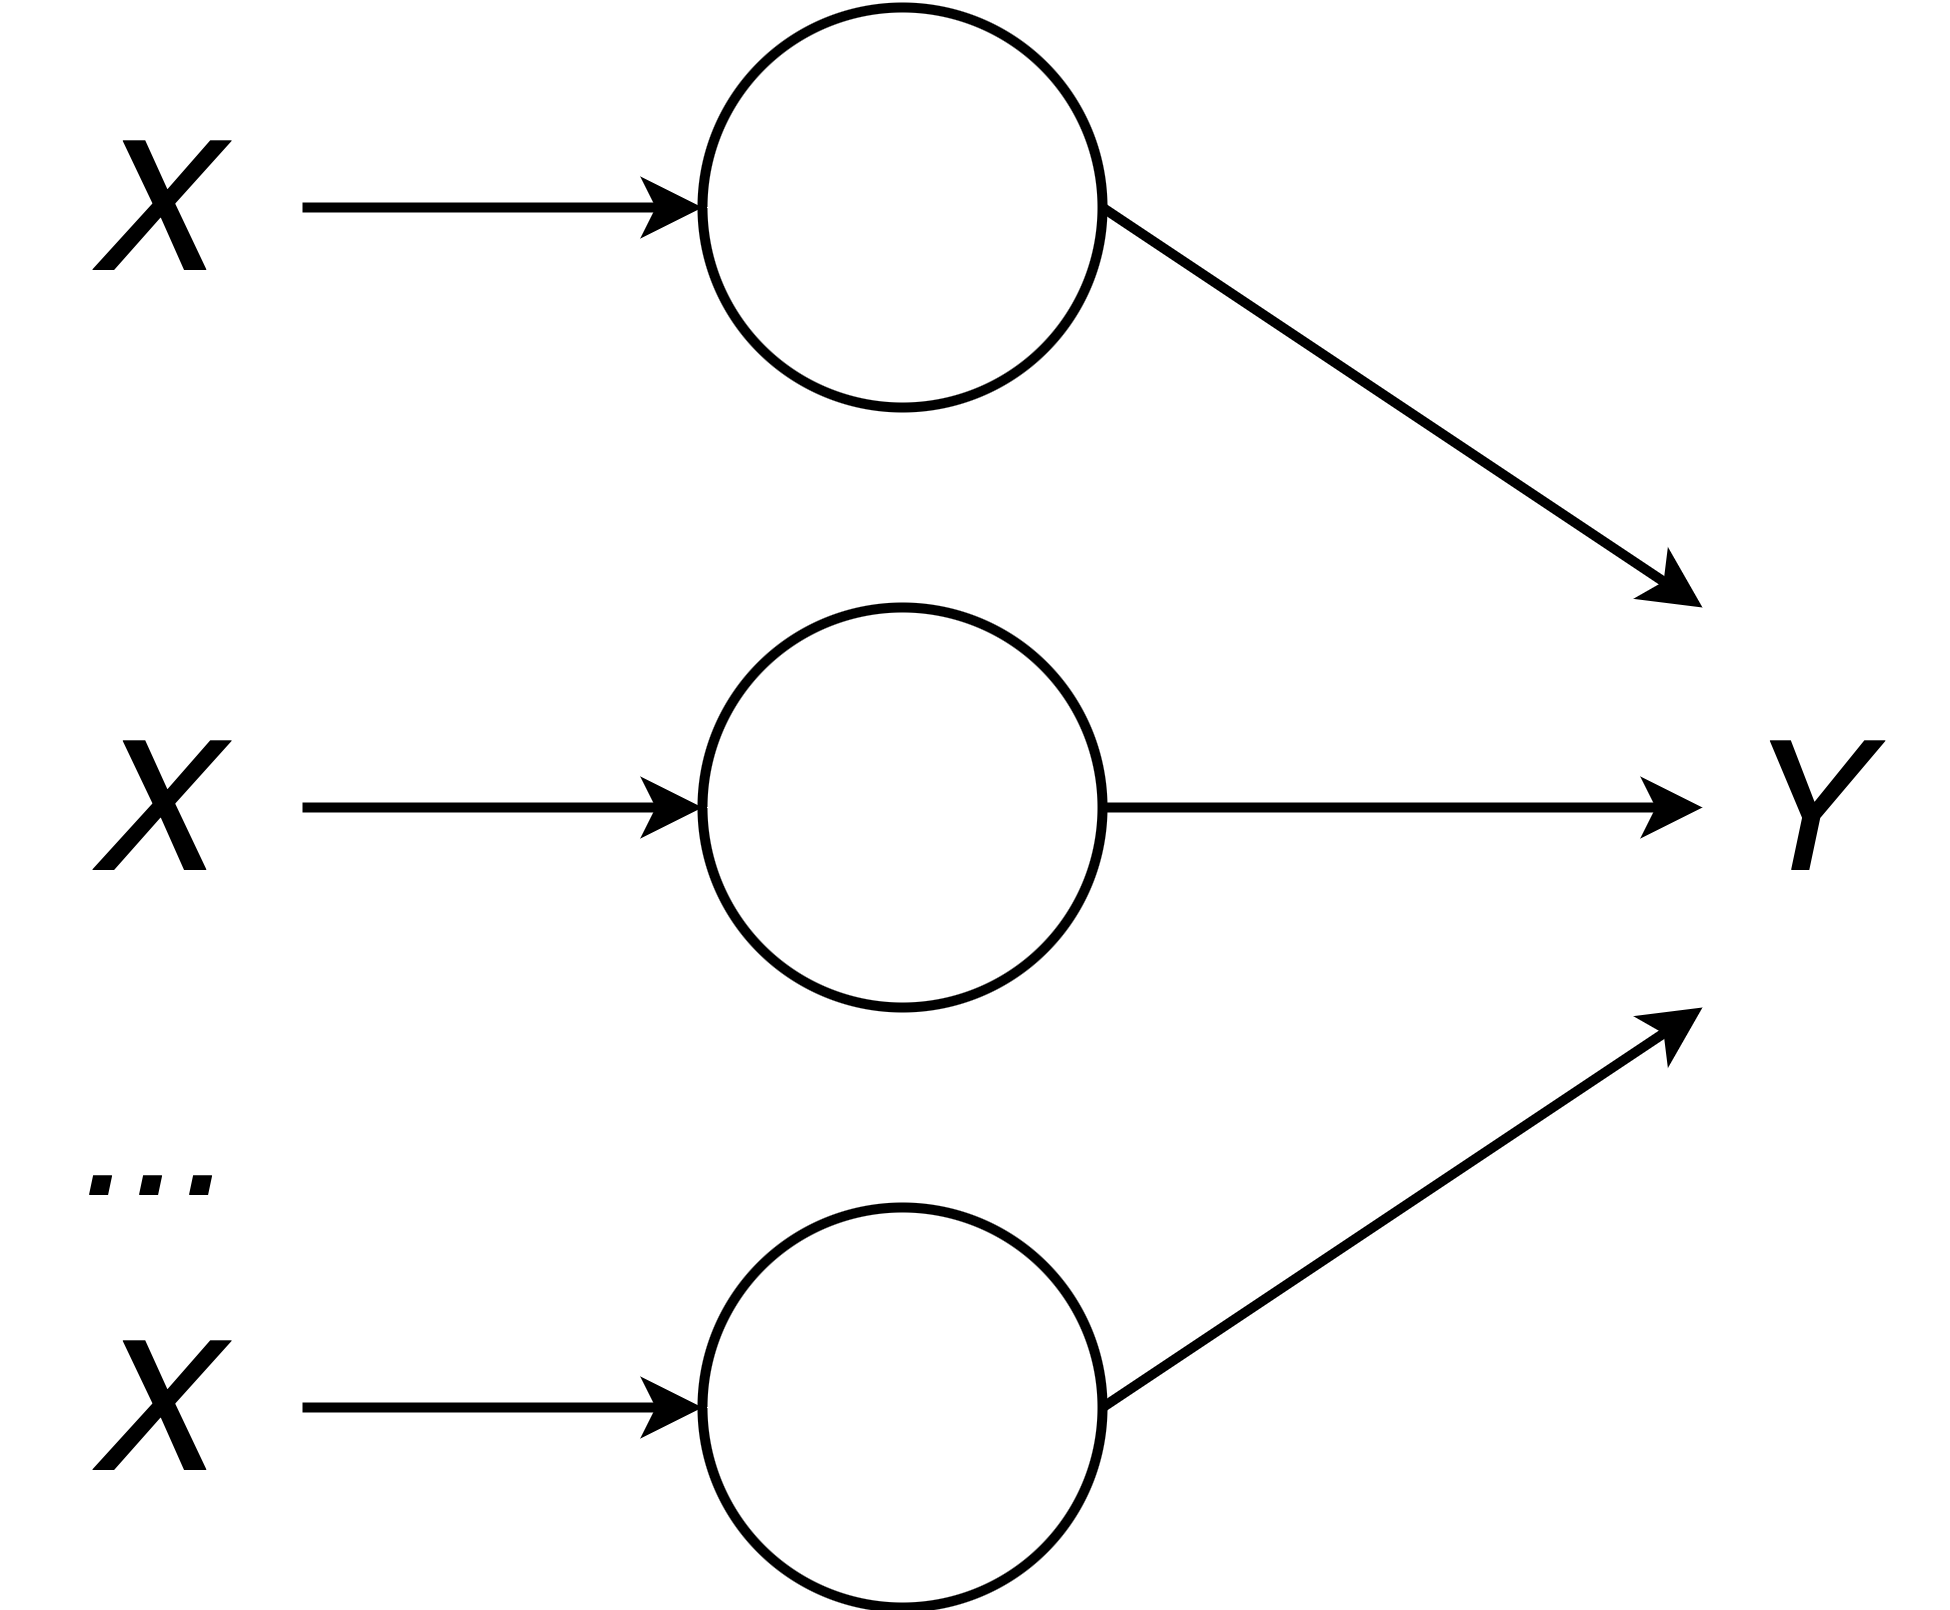
\includegraphics[width=0.6\textwidth]{man-source/images/ch1/pic0-2.png}
  \caption{Слой нейронных элементов}
  \label{fig:pic0_2}
\end{figure}

Наконец, слои нейронных элементов объединяются в последовательности, формируя общую архитектуру нейронной сети (последовательность слоев, их тип, количество нейронов в каждом слое, функцию активации и другие характеристики). Итоговая модель способна выполнять аппроксимацию любой непрерывной функции с любой точностью после выполнения обучения \cite[c.~312]{Cybenko1989ApproximationBS}. В процессе обучения данные из некоторой выборки подаются на вход сети с целью определения градиентов изменения параметров нейронных элементов. Одна итерация, в ходе которой модели предъявляются все обучающие примеры, называется эпохой. Данная процедура выполняется до тех пор, пока не будет достигнут ответ сети, полученный с желаемой точностью или пока весовые коэффициенты не войдут в некоторое стационарное состояние. 

Искусственные нейронные сети могут быть классифицированы по различным признакам (например, по характеру обучения, по направлению связей, по архитектуре и так далее). В литературе часто используется классификация по архитектурному признаку. Согласно ей, выделяют \cite[c.~24-25]{golovko2017}:

\begin{easylistNum}
    & сети персептронного типа (многослойные персептроны \cite[c.~92-94]{ivakhnenko1967cybernetics}, рекуррентные [\citen{Elman1990FindingSI}, c.~182-185; \citen{Jordan86}, c.~5-6], рециркуляционные \cite[c.~360-361]{Hinton1987LearningRB}, сверточные [\citen{fukushima1980}, c.~194-197; \citen{LeCun1989HandwrittenDR}, c.~398-402], глубокие);
    & самоорганизующиеся НС (НС Кохонена \cite[c.~105-106]{kohonen2001}, сети адаптивного резонанса \cite[c.~33-34]{Grossberg1987CompetitiveLF});
    & релаксационные НС (сети Хопфилда \cite[c.~3089]{Hopfield1984}, Хэмминга \cite[c.~8-10]{Lippmann1987} и двунаправленная ассоциативная память \cite[c.~52-54]{Kosko1988BidirectionalAM});
    & гибридные НС (сети встречного распространения \cite{HechtNielsen1987}, RBF-сети \cite[c.~326-327]{Broomhead1988}, нечеткие сети \cite{Jang1997});
    & нейронные иммунные сети \cite[c.~485]{Golovko2010}.
\end{easylistNum}

В данной работе исследуются глубокие нейронные сети, являющиеся развитием архитектур полносвязных сетей (персептронов) и сверточных нейронных сетей.

В настоящий момент сверточные нейронные сети и глубокие архитектуры на их основе являются доминирующими в области компьютерного зрения \cite[c.~436]{LeCun2015}. В основном это связано с тем, что в подобных задачах используются данные с высокой корреляцией между соседними элементами (для цифровых фотографий и видео в качестве этих значений выступают массивы пикселей), а сверточные слои особенно эффективны при обработке именно таких данных \cite[c.~8]{Emmert2020}.

Сверточные нейронные сети базируются на моделях неокогнитрона, предложенной К. Фукусимой \cite[c.~193]{fukushima1980}, и сетях с разделяемыми весами. Первая классическая модель сверточной нейронной сети была разработана ЛеКуном и получила название LeNet-5 \cite[c.~7]{lekun1998}. Сверточные нейросети интегрировали три концепции, называемые локальным рецептивным полем, разделяемыми весовыми коэффициентами и пространственной подвыборкой. Используя локальное рецептивное поле, нейронные элементы первого сверточного слоя могут извлекать простейшие признаки, такие как края, углы и так далее. Первые слои сверточной нейронной сети представляют собой комбинацию сверточных (convolutional) и подвыборочных (pooling) слоев (рисунок \ref{fig:cnn_common_view}), благодаря чему осуществляется нелинейное иерархическое преобразование входной информации. При решении задачи классификации в качестве последнего слоя могут использоваться SVM-классификатор, многослойный персептрон или любой другой классификатор (на рисунке обозначен как classifier).

\begin{figure}[ht]
	\centering
	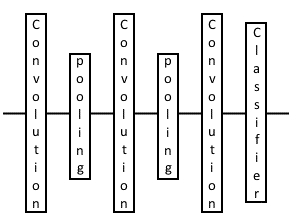
\includegraphics[width=14cm]{man-source/images/ch4/pic4-15.png}
	\caption{Общий вид сверточной нейронной сети}
	\label{fig:cnn_common_view}
\end{figure}
Таким образом, сверточные модели могут включать как сверточные слои, так и некоторое количество полносвязных слоев (завершающие полносвязные слои часто используются как классификаторы признаков, извлеченных на начальных сверточных слоях). %Таким образом, исследование и обучение полносвязных архитектур остается актуальной задачей. 

Несмотря на лидирующее положение сверточных сетей, полносвязные архитектуры также успешно применяются для некоторых задач компьютерного зрения (например, при решении задачи трехмерной реконструкции \cite[c.~10]{mildenhall2020nerf}). Далее в работе будет показано, что сверточный слой может быть представлен с помощью разряженного слоя. Таким образом, исследование и обучение полносвязных архитектур остается актуальной задачей. 

Глубокую нейронную сеть можно определить как искусственную нейронную сеть персептронного типа, имеющую более двух скрытых слоев нейронных элементов.

В общем случае глубокая нейронная сеть (deep neural network -- DNN) представляет собой нейросетевую модель с множеством слоев нейронных элементов \cite[c.~59]{Golovko2015a}. Рассмотрим многослойный персептрон -- полносвязную нейросетевую модель, представленную на рисунке~\ref{fig:pic1_1}). Известно, что такая сеть способна к выделению глубокой иерархии признаков \cite[c.~3]{n5}. 

\begin{figure}[H]
  \centering
  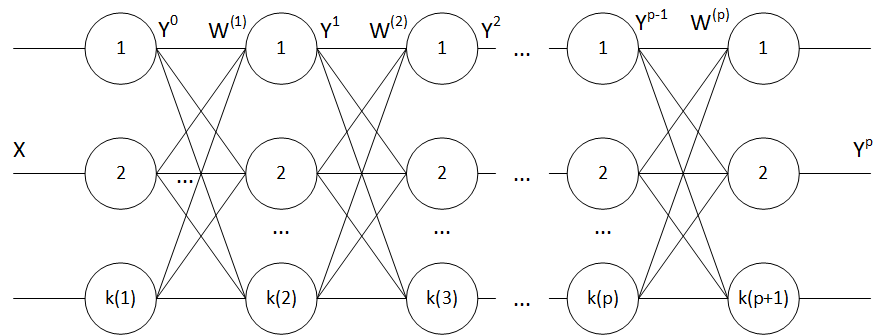
\includegraphics[width=\textwidth]{man-source/images/ch1/pic1-1.png}
  \caption{Глубокая нейронная сеть}
  \label{fig:pic1_1}
\end{figure}

На первом скрытом слое выделяются признаки низкого уровня абстракции, на втором слое -- более высокого уровня и так далее \cite{n3}. 

Выходное значение $j$-го нейрона $k$-го слоя определяется следующим образом:

\begin{equation}
y_j^k=F(S_j^k),
\end{equation}

\begin{equation}
S_j^k=\sum_{i=1} w_{ij}^ky_i^{k-1}+T_j^k,
\end{equation}
где $F(\cdot)$ -- функция активации нейронного элемента \textit{k}-го слоя,\\
$S_j^k$ -- взвешенная сумма $j$-го нейрона $k$-слоя,\\
$w_{ij}^k$ -- весовой коэффициент между $i$-ым нейроном ($k$-1)-го слоя и $j$-м нейроном $k$-го слоя,\\
$T_j^k$ -- пороговое значение $j$-го нейрона $k$-го слоя.

Для первого слоя НС, называемого распределительным, справедливо		
\begin{equation}
y_j^0=x_j.
\end{equation}

В матричном виде выходной вектор $k$-го слоя 

\begin{equation}
Y^k=F(S^k)=F((Y^{k-1})^TW^k+T^k),
\end{equation}
где $W^k$ -- матрица весовых коэффициентов $k$-го слоя,\\
$Y^{k-1}$ -- выходной вектор-столбец ($k$-1)-го слоя,\\
$T^k$ -- вектор пороговых значений нейронов $k$-го слоя.

Если глубокая нейронная сеть используется для классификации образов, то выходные значения сети часто определяются на основе функции активации \textbf{softmax} \cite[c.~34]{golovko2017}: 		

\begin{equation}
y_j^F=softmax(S_j)=\frac{e^{S_j}}{\sum_i e^{S_i}}.
\end{equation}
В этом случае значения, получаемые на последнем слое нейронной сети, отражают вероятность принадлежности данного образа к определенному классу.

\section{Проблемы обучения глубоких моделей}

Теория нейронных сетей не развивалась равномерно. Нередко причинами приостановок в исследованиях являлось отсутствие доступных на определенный момент времени эффективных методов обучения моделей. 

Начиная с первых моделей ИНС, описанных в работе У. Мак-Каллока и У. Питтса \cite[c.~105]{mcculloch43a} в 1943 году, искусственным нейронным сетям были посвящены концептуальные и важные работы того времени (например, правила обучения Д. Хебба \cite[c.~62]{hebb1949}, В. Видроу и М. Хоффа \cite[c.~99]{widrow1960}). В 1959 году Ф. Розенблатт предложил модель персептрона \cite[c.~99]{Rosenblatt1962}. Однако, после опубликования монографии М. Минского и С. Пайперта <<Персептроны>> в 1969 году \cite[c.~249]{minsky69perceptrons} крупные исследования в этой области были приостановлены. В этой работе был проведен анализ персептронной модели и выявлены ее основные ограничения, в том числе касающиеся невозможности эффективного решения существующими на тот момент моделями некоторых задач (например, задач инвариантного представления образов). %Это повлияло на развитие нейронных сетей и, вплоть до 1985 года, теория не развивалась. 

В конце 1970-х годов произошел очередной всплеск работ, посвященных нейросетевым моделям (например, сетям адаптивного резонанса \cite[c.~187]{Grossberg1976}, ассоциативной памяти \cite[c.~69]{Kohonen1977}).
В 1986 году Д. Румельхартом, Дж. Хинтоном и Р. Вильямсом в работе \cite[c.~4-8]{rumelhart1986learning} был предложен метод обратного распространения ошибки для обучения многослойных моделей. Результаты, изложенные в данной работе, открыли теоретические возможности для обучения моделей с большим количеством слоев.  Однако, вплоть до середины 2000-х годов сети с количеством слоев три и более широко не применялись, так как считалось, что использование глубоких моделей не дает существенного прироста в эффективности по сравнению с другими подходами. Неэффективность была связана с проблемой <<исчезающего>> градиента. Она проявляется в том, что при обучении ГНС методом обратного распространения ошибки значения градиентов весовых коэффициентов первых слоев сети быстро становятся близкими к нулю, в результате весовые коэффициенты таких слоев практически не изменяются \cite[c.~38]{n5}. Это существенно замедляет процесс обучения, делая невозможным практическое применение подобных моделей по сравнению с другими существовавшими на тот момент времени методами (например, \cite[c.~274]{Corinna1995}).

Тем не менее, проводя аналогии с многоуровневыми нейронными архитектурами в человеческом мозге (в частности, строением вентральной зрительной системы), было понятно, что подобный тип искусственных нейронных сетей обладает полезными свойствами, позволяя формировать многоуровневую иерархию признаков \cite[c.~66]{Behnke2003}.

В 2006 году Джеффри Хинтоном был предложен подход к обучению глубоких моделей, который ознаменовал начало новой эпохи в развитии теоретических работ в данной области \cite[c.~1533-1538]{n1}.

В предложенном методе использовался <<жадный>> алгоритм послойного предобучения глубоких нейронных сетей (greedy layer-wise algorithm) \cite[c.~3-4]{Hinton2009}, основанный на применении ограниченных машин Больцмана, последовательно формируемых и обучаемых из слоев глубокой нейронной сети. 

С этой работы фактически начался новый подъем в исследованиях нейронных сетей, который длится до настоящего времени. За последующие годы в области компьютерного зрения благодаря применению глубоких нейронных сетей удалось значительно улучшить результаты для различных задач, включая классификацию, детекцию, сегментацию объектов на изображении, генерацию текстовых описаний к изображениям, генерацию изображений по текстовым описаниям и т.д.  % Последовавший всплеск количества работ, посвященных обучению и применению глубоких сетей в различных сферах, позволил в течение последующих нескольких лет значительно улучшить первоначальные результаты.

В течение следующих лет сместился основной акцент в исследованиях -- вместо послойного обучения стали применяться методы, позволяющие обучать глубокие нейронные сети, начиная с произвольной начальной инициализации, без использования предобучения (например, стохастический градиентный спуск с использованием функции активации ReLU и ее вариантов \cite[c.~318]{glorot2011}). Однако, применение таких подходов не снижает требований к объему обучающей выборки, которая в идеальных теоретических условиях должна быть сравнима с числом настраиваемых параметров модели, поскольку большие модели, обучаемые на малых выборках, с большей вероятностью будут переобучаться. Результатом этого является отличная приспособленность модели к обучающей выборке, но плохая обобщающая способность, т.е. неэффективность сети на тестовых данных. Таким образом, объем используемой обучающей выборки для глубоких нейронных сетей остается по-прежнему критичным фактором для обучения. Даже наличие подходящей по объему выборки не гарантирует успешное завершение обучения, так как подготовка больших моделей может повлечь неприемлемые аппаратные издержки [\citen{alpaca2023}; \citen{alpacagithub}; \citen{zhang2022opt}, c.~1].

\section{Методы обучения}

Рассмотрим основные методы, применяемые для обучения ГНС.

Существуют два базовых подхода к обучению глубоких нейронных сетей, оба из которых включают этап предобучения:

\begin{easylistNum}    
    & обучение с использованием предобучения на большой обучающей выборке и любого оптимизирующего метода для настройки параметров нейронной сети (I тип);
	& обучение с использованием неконтролируемого предобучения (II~тип).
\end{easylistNum}

Предобучение I типа представляет собой обучение модели с использованием метода обратного распространения ошибки, некоторого оптимизирующего метода и активационных функций ReLU и ее вариантов в качестве функций активации нейронов \cite[c.~436-438]{LeCun2015}, а затем дообучение полученной модели для новой выборки (transfer learning). 

Среди основных оптимизирующих методов, применяемых для предобучения I типа, выделяют \cite[c.~263-266]{Goodfellow2017}:

\begin{easylistNum}
	& SGD (стохастический градиентный спуск). В данном методе корректировка настраиваемых параметров ИНС выполняется в направлении, противоположном вектору градиента функции потерь \cite[c.~225-237]{Haykin2006};
	& метод Нестерова. Обучение методом стохастического градиентного спуска нередко происходит очень медленно. Метод Нестерова является вариантом импульсного алгоритма, в котором градиент вычисляется после применения текущей скорости \cite[c.~258]{Goodfellow2017}. Применение импульсного метода помогает ускорить процесс обучения в случаях зашумленных или небольших по величине градиентов;
	& AdaGrad. В данном методе осуществляется независимая адаптация скоростей обучения всех настраиваемых параметров ИНС \cite[c.~2124-2125]{Duchi2011};
	& RMSProp. Данный метод является модификацией AdaGrad, которая позволяет улучшить его поведение в случае невыпуклой целевой функции \cite[c.~1]{hintonlecture2012};
	& Adam. Данный метод можно рассматривать как комбинацию RMSProp и AdaGrad \cite[c.~5]{Kingma2014}. 
	Помимо усредненного первого момента, данный метод использует усредненное значение вторых моментов градиентов.
\end{easylistNum}

I тип фактически представляет собой обучение с нуля, которое осуществляется на больших выборках данных с использованием подходящих аппаратных средств. Предобученные таким образом модели могут быть использованы для решения других задач. Таким образом, современный инженер получает в свое распоряжение репозиторий готовых предобученных моделей, которые могут быть дообучены на небольших выборках данных, предназначенных для решения конкретной задачи.

Рассмотрим подробно реализацию предобучения II типа.

Исследование методов предобучения II типа остается актуальной и перспективной задачей, поскольку такие методы позволяют существенно сократить размер применяемой обучающей выборки, при этом не переобучая модель \cite[c.~439]{LeCun2015}. Эффектом, достигаемым за счет данного свойства, является снижение требований к используемому для обучения оборудованию.

Обучение нейронной сети с предобучением II типа можно разделить на два этапа [\citen{n3}; \citen{n1}, c.~1538; \citen{n2}, c.~18]: 
\begin{easylistNum}
	& этап предобучения НС методом послойного обучения (pre-training). Осуществляется неконтролируемо;
	& дообучение (fine-tuning) при помощи алгоритмов <<бодрствования и сна>> (wake-sleep algorithm) \cite[c.~2]{hinton1995} или обратного распространения ошибки.
\end{easylistNum}

В ходе \textbf{первого этапа} осуществляется инициализация параметров нейросетевой модели. Данный этап является определяющим для последующего дообучения модели.
Для реализации первого этапа используются два основных подхода (рисунок~\ref{fig:pic1_2}).
Формирование вспомогательных моделей (ограниченных машин Больцмана, автоэнкодеров) в обоих подходах происходит из структуры исходной НС. 

\begin{figure}[H]
  \centering
  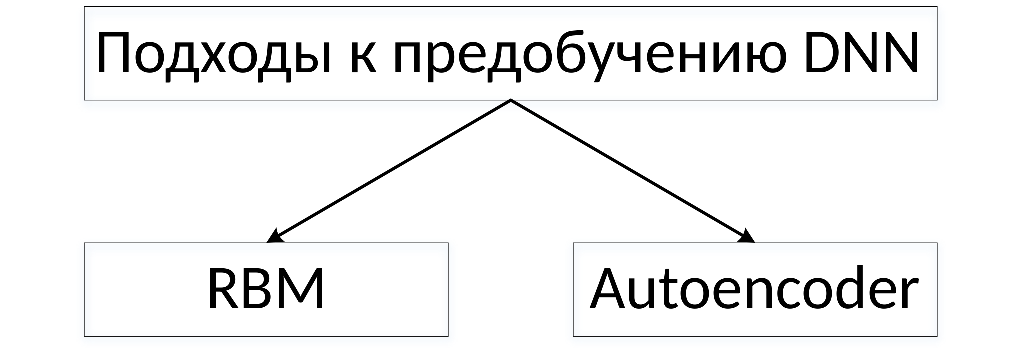
\includegraphics[width=0.7\textwidth]{man-source/images/ch1/pic1-2.pdf}
  \caption{Методы предварительного обучения ГНС}
  \label{fig:pic1_2}
\end{figure}

Первый подход основывается на представлении каждого слоя нейронной сети в виде ограниченной машины Больцмана (RBM). При использовании автоэнкодерного подхода, каждый слой представляется автоассоциативной нейронной сетью.

Рассмотрим каждый из этих методов подробнее.

\def\slantfrac#1#2{ \hspace{3pt}\!^{#1}\!\!\hspace{1pt}/
  \hspace{2pt}\!\!_{#2}\!\hspace{3pt}
}

При предобучении ГНС в соответствии с \textbf{первым подходом} осуществляется построение последовательности RBM-сетей из параметров скрытых слоев ГНС и их обучение. 

Ограниченная машина Больцмана состоит из двух слоев стохастических бинарных нейронных элементов, соединенных между собой двунаправленными симметричными связями (рисунок~\ref{fig:pic1_3}). Входной слой нейронов называется видимым (слой $X$), а выходной -- скрытым (слой $Y$). Ограниченная машина Больцмана может генерировать любое дискретное распределение, если используется достаточное число нейронов скрытого слоя \cite[c.~57]{n5}.

\begin{figure}[H]
  \centering
  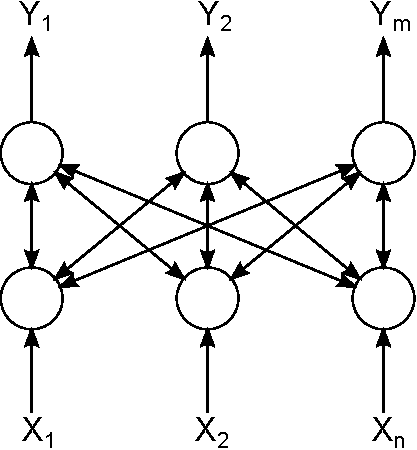
\includegraphics[width=0.4\textwidth]{man-source/images/ch1/pic1-3.pdf}
  \caption{Ограниченная машина Больцмана}
  \label{fig:pic1_3}
\end{figure}	

В данной модели состояния видимых и скрытых нейронов меняются в соответствии с вероятностной версией сигмоидной функции активации:
	
\begin{equation}
	p(y_j\lvert x)=\frac{1}{1+e^{-S_j}},\ S_j=\sum_i^n w_{ij}x_i+T_j,
\end{equation}
	
\begin{equation}
	p(x_i\lvert y)=\frac{1}{1+e^{-S_i}},\ S_i=\sum_j^m w_{ij}y_j+T_i,
\end{equation}
где $S_i, S_j$ -- взвешенные суммы видимого и скрытого слоев,\\
$T_i, T_j$ -- пороговые элементы видимого и скрытого слоев соответственно.
	
Состояния видимых и скрытых нейронных элементов принимаются независимыми:
	
\begin{equation*}
\begin{aligned}
	P(x \lvert y) = \prod_{i=1}^n P(x_i \lvert y),\\
	P(y \lvert x) = \prod_{j=1}^m P(y_j \lvert x).
\end{aligned}	
\end{equation*}
	
Таким образом, состояния всех нейронов ограниченной машины Больцмана определяются через распределение вероятностей. В RBM нейроны скрытого слоя являются детекторами признаков, которые сохраняют закономерности входных данных. Основная задача обучения состоит в воспроизведении распределения входных данных на основе состояний нейронов скрытого слоя как можно точнее. Для достижения этого применяется процедура CD-\textit{k}. В главе 2 будет подробно описана данная процедура и приведен вывод классических правил обучения RBM. %Это эквивалентно  максимизации функции правдоподобия путем модификации синаптических связей нейронной сети. Покажем основные этапы вывода правил обучения для RBM.

При предобучении ГНС на базе RBM (в процессе первого этапа обучения) вначале создается RBM-модель из первого скрытого слоя ГНС. Для данной RBM входные данные поступают на видимый слой нейронных элементов и используя CD-$k$ процедуру вычисляются состояния скрытых $P(y \lvert x)$ и видимых нейронов $P(x \lvert y)$. В процессе выполнения данной процедуры в течение заданного количества эпох изменяются весовые коэффициенты и пороговые значения сети RBM, которые затем фиксируются. Следующим берется второй скрытый слой глубокой нейронной сети и конструируется новая RBM. Входными данными для нее являются данные с предыдущего слоя (выходные данные, полученные первой RBM). Выполняется обучение новой модели и процесс продолжается для всех последующих слоев нейронной сети, за исключением, возможно, самого последнего (включение последнего слоя в процесс предобучения зависит от решаемой задачи -- например, для задачи классификации предобучение последнего слоя не требуется, так как он должен обучаться с учителем), как показано на рисунке~\ref{fig:pic1_4}. 

\begin{figure}[H]
  \centering
  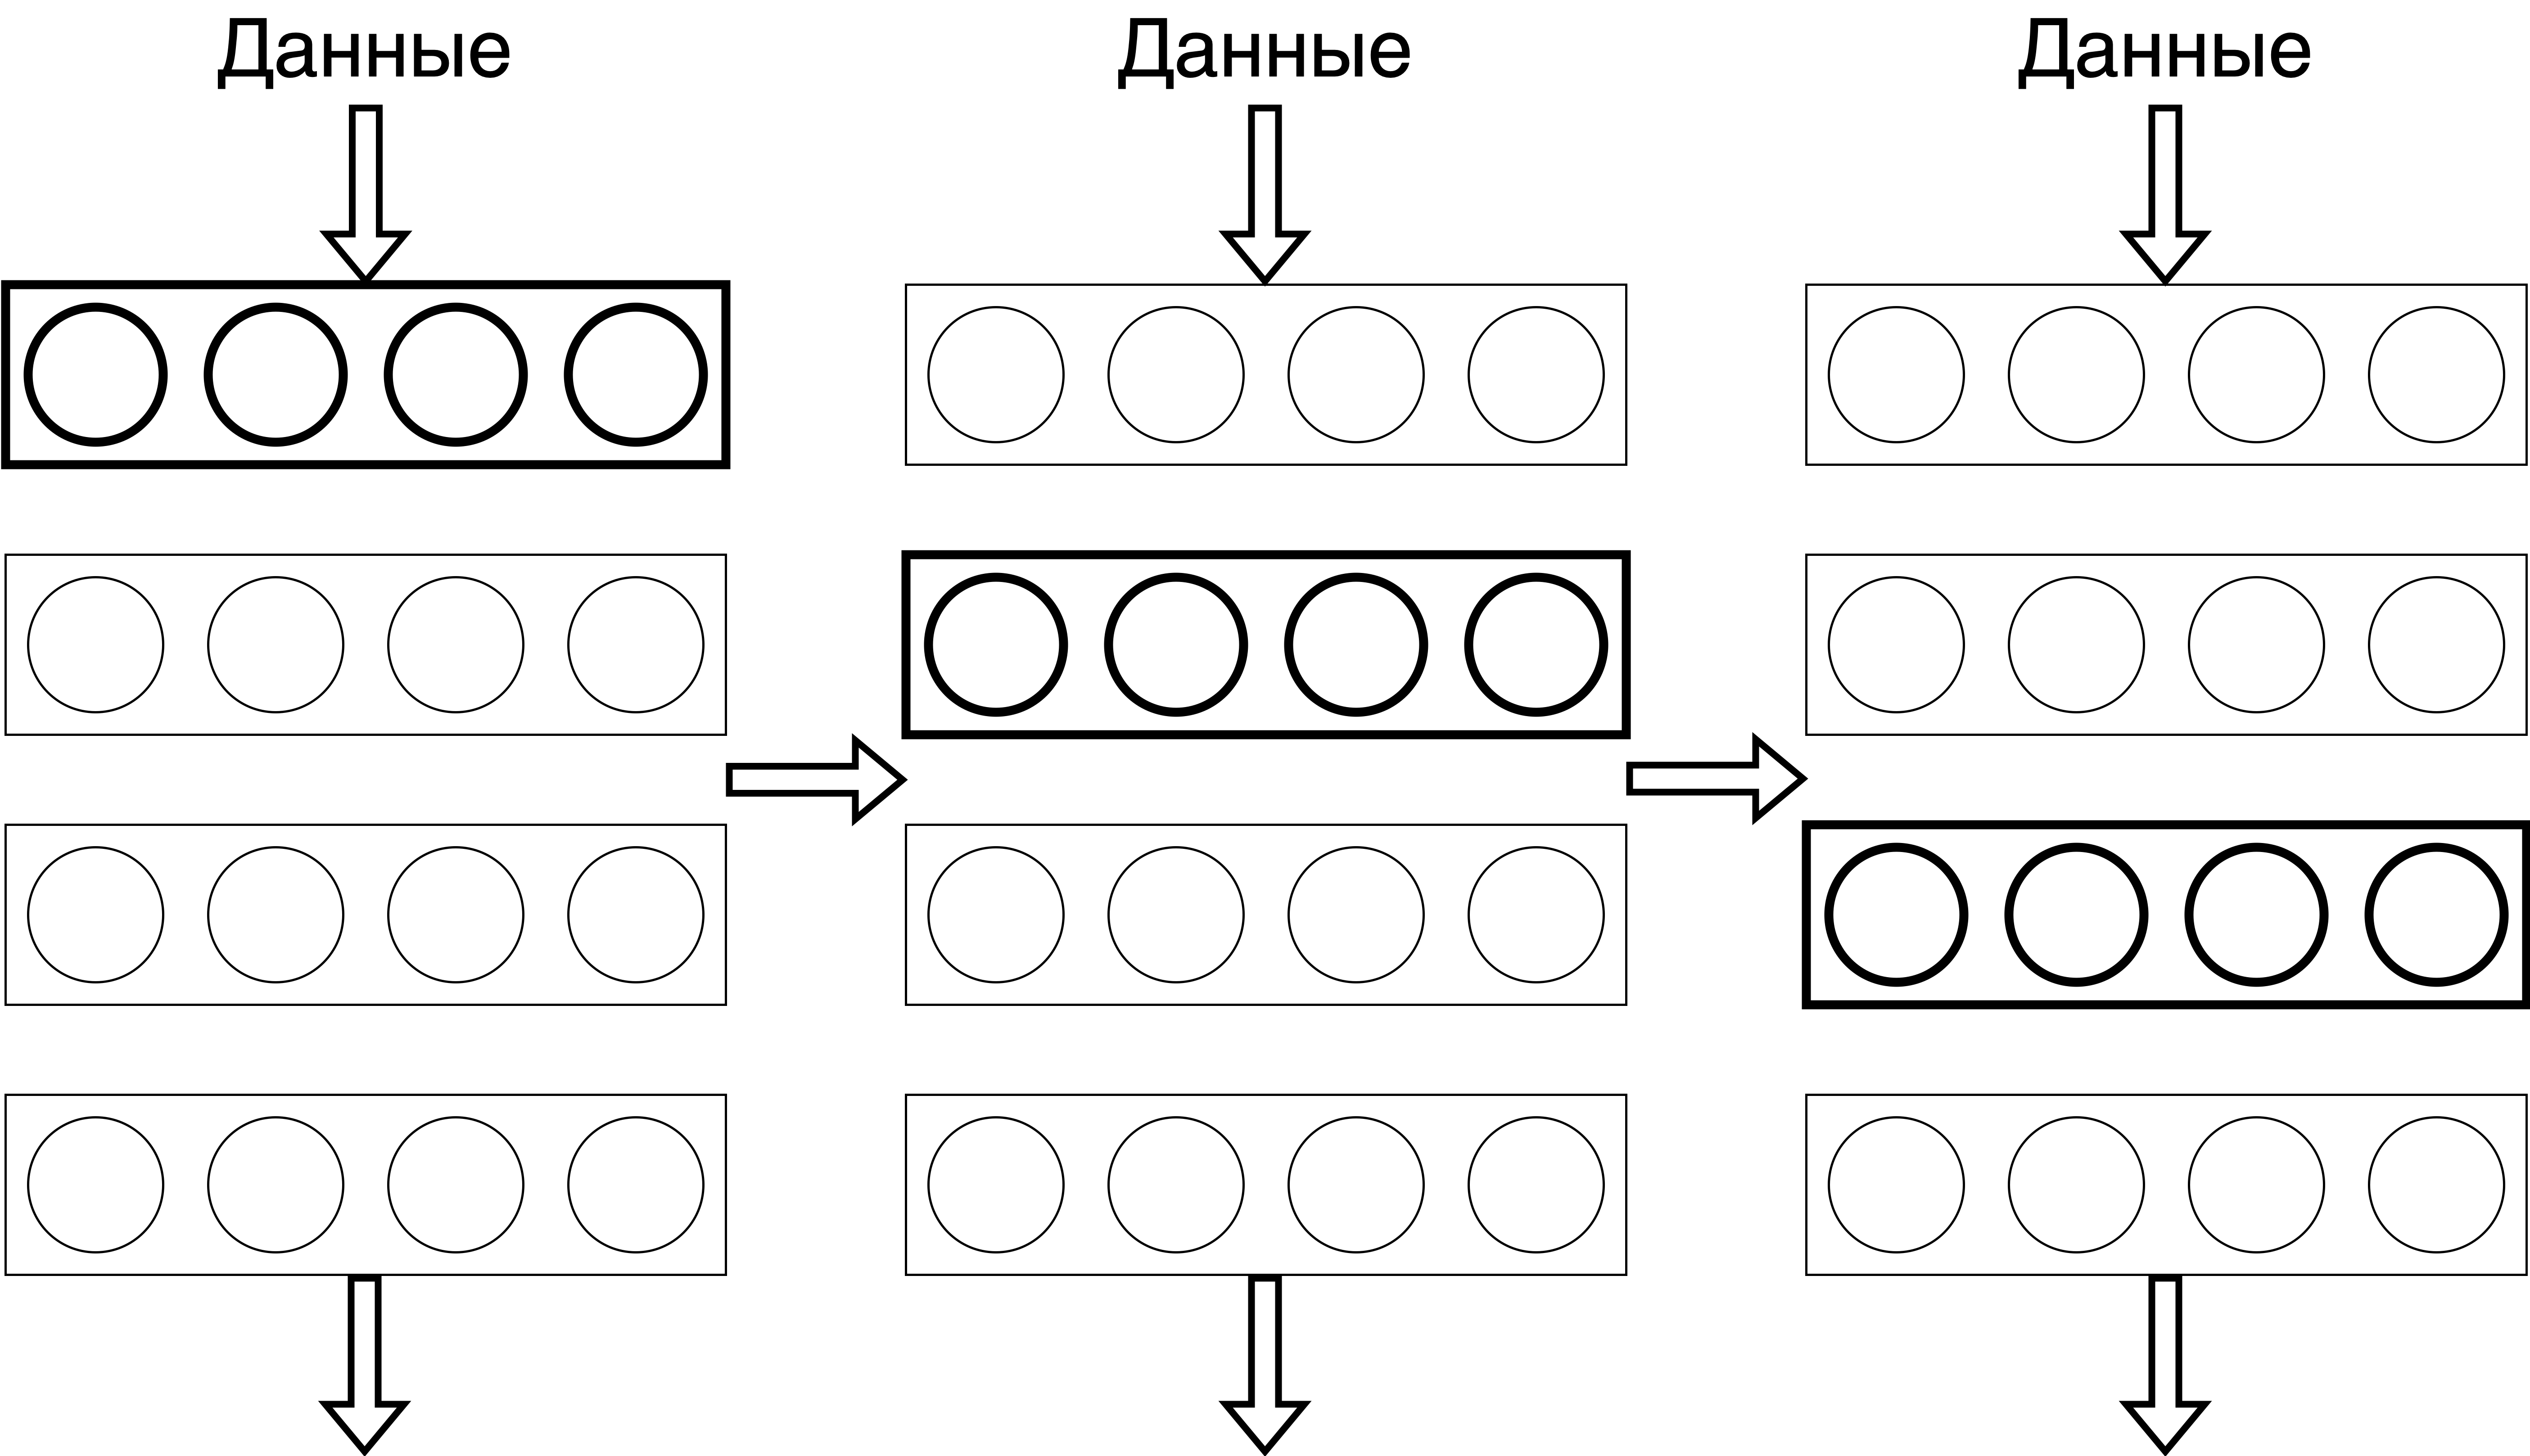
\includegraphics[width=\textwidth]{man-source/images/ch1/pic1-4.png}
  \caption{<<Жадный>> алгоритм послойного обучения}
  \label{fig:pic1_4}
\end{figure}

При предобучении ГНС в соответствии со \textbf{вторым подходом} \cite[c.~158]{n6}, вначале обучается первый слой ГНС как автоассоциативная нейронная сеть с целью минимизации суммарной ошибки реконструкции данных, затем обучается второй слой ГНС и так далее. Для обучения каждого слоя можно использовать алгоритм обратного распространения ошибки. 
	
Рассмотрим персептрон с тремя скрытыми слоями (рисунок \ref{fig:pic1_5}). Тогда в соответствии с автоэнкодерным методом, прежде всего, берутся первые два слоя нейронной сети (1 и 2) и на базе их конструируется автоассоциативная (рециркуляционная) нейронная сеть (1-2-1), то есть добавляется восстанавливающий слой (рисунок \ref{fig:pic1_6}). 
	
\begin{figure}[H]
  \centering
  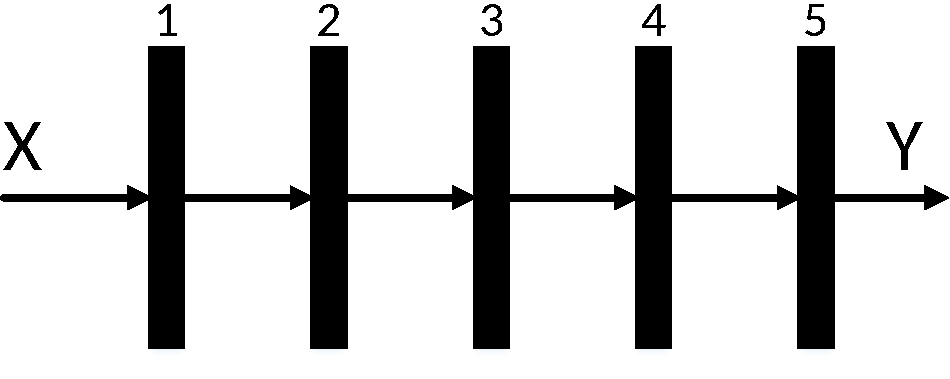
\includegraphics[width=0.7\textwidth]{man-source/images/ch1/pic1-5.pdf}
  \caption{Персептрон с тремя скрытыми слоями}
  \label{fig:pic1_5}
\end{figure}	

\begin{figure}[H]
  \centering
  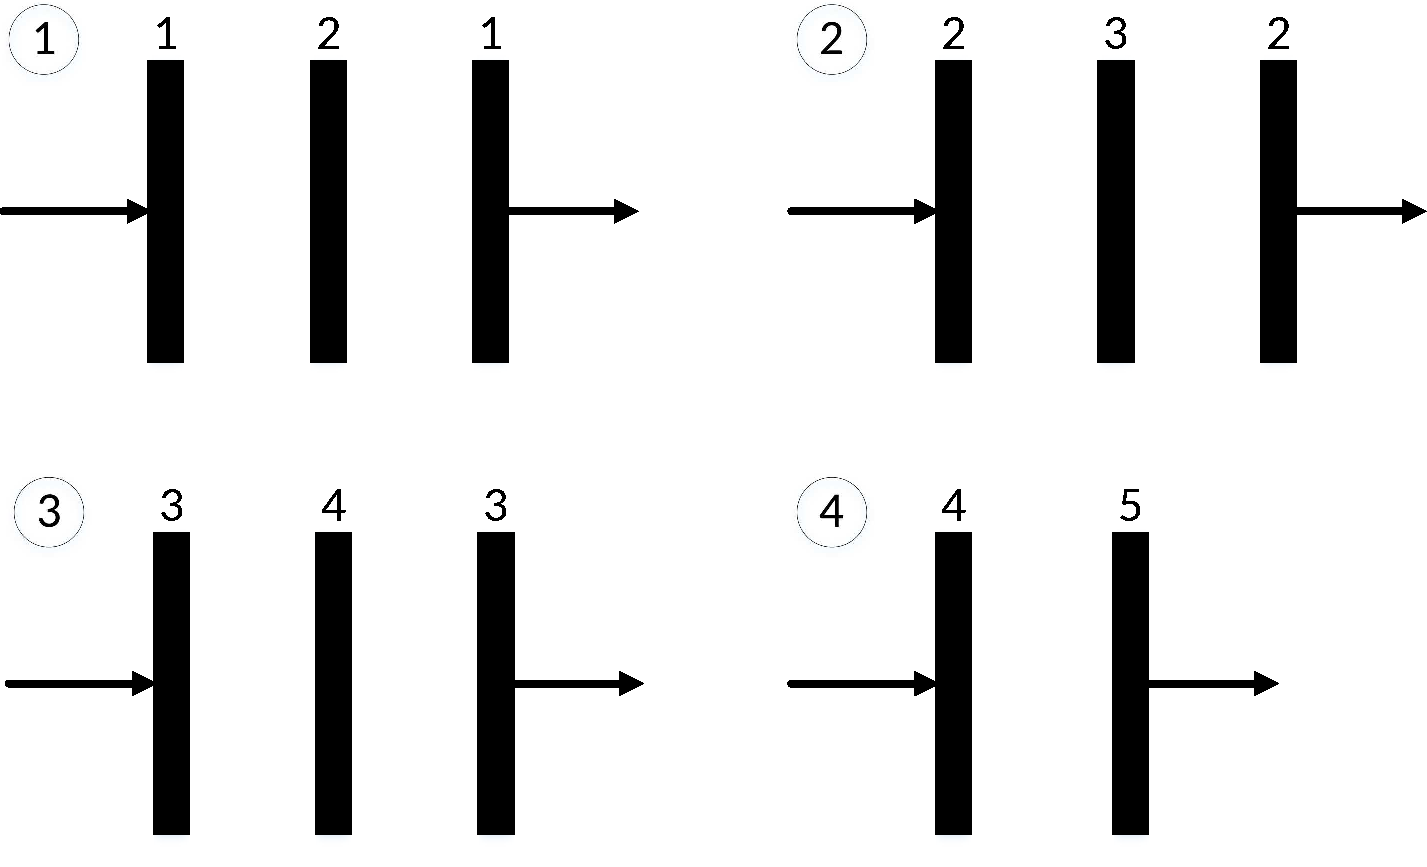
\includegraphics[width=0.7\textwidth]{man-source/images/ch1/pic1-6.pdf}
  \caption{Автоэнкодерный метод обучения}
  \label{fig:pic1_6}
\end{figure}

Затем, происходит обучение такой сети, например, при помощи алгоритма обратного распространения ошибки с целью минимизации ошибки реконструкции данных. 
	
После этого отбрасывается восстанавливающий слой (последний слой) автоассоциативной сети, фиксируются веса скрытого слоя, и конструируется автоассоциативная сеть из следующих двух слоев нейронной сети (2-3-2), которая обучается на основе данных, поступающих с предыдущего (2-го слоя). Процесс продолжается до последнего или предпоследнего слоя, как это схематично изображено на рисунке \ref{fig:pic1_6}. %В результате послойного обучения получается предварительно обученная нейронная сеть. Далее осуществляется точная настройка (fine-tuning) посредством, например, алгоритма обратного распространения ошибки с учителем.
	
Данный процесс можно представить в виде следующего алгоритма:
\begin{easylistNum}
	& конструируется автоассоциативная сеть с входным слоем $X$, скрытым $Y$ и выходным слоем $X$;
	& обучается автоассоциативная сеть, например при помощи алгоритма обратного распространения ошибки и фиксируются синаптические связи первого слоя $W_1$;
	& берется следующий слой глубокой нейронной сети и снова формируется автоассоциативная сеть аналогичным образом;
	& используя настроенные синаптические связи предыдущего слоя $W_1$, подаются входные данные на вторую автоассоциативную сеть и она обучается аналогичным образом. В результате получаются весовые коэффициенты второго слоя $W_2$;
	& процесс продолжается до последнего или предпоследнего слоя нейронной сети.
\end{easylistNum}

Для обоих подходов (RBM и автоэнкодерный), с помощью реализации такого неконтролируемого предобучения можно получить приемлемую начальную инициализацию настраиваемых параметров глубокой нейронной сети. 

На \textbf{втором этапе}, иначе называемом этапом <<тонкой настройки>> нейронной сети или fine-tuning, выполняется дообучение всей глубокой модели с использованием, например, алгоритма <<бодрствования и сна>> или обратного распространения ошибки.

Критически важным для этого этапа является начальная инициализация весов и порогов. Если такая инициализация выполнена в ходе предобучения, то сеть начинает процесс <<тонкой настройки>> с <<хороших>> начальных значений, что обуславливает быструю сходимость.

Если же предобучение отсутствует и используется традиционная <<поверхностная>> схема обучения со случайной инициализацией параметров, обучение сети может быстро остановиться и, как результат, приемлемая обобщающая способность не будет достигнута.

В дальнейшем под предобучением будем понимать предобучение II~типа, проводимое с использованием RBM-сетей, если не указано иного. 

\section{Критерии минимизации при обучении}

При обучении ГНС (например, на этапе <<тонкой настройки>>, если сеть предобучалась) важно определить критерий минимизации. Наиболее известными и используемыми в настоящий момент функциями ошибок являются функция квадратичной ошибки (SE)

\begin{equation}
	\label{MSE}
	E_{SE} = \frac{1}{2}\sum_{j=1}^{n}(y_j - t_j)^2
\end{equation}
и кросс-энтропийная функция (CE) -- случай мультиклассовой классификации

\begin{equation}
	\label{CE_multiclass}
	E_{CE_{mult}} = -\sum_{j=1}^{n}t_j\log(y_j),
\end{equation}
где $n$ -- количество нейронных элементов в последнем слое,\\
$y_j$ -- выход нейрона $j$,\\
$t_j$ -- эталонное значение этого нейрона,\\
множитель $\frac{1}{2}$ введен для удобства вычислений.

Формула \ref{MSE} справедлива для одного обучающего примера. Для $L$ обучающих примеров она запишется в следующем виде (MSE -- среднеквадратичная ошибка):

\begin{equation}
	\label{MSE_L}
	E_{MSE} = \frac{1}{2L}\sum_{k=1}^{L}\sum_{j=1}^{n}(y_j^k - t_j^k)^2.
\end{equation}

При обучении автоэнкодеров часто применяется кросс-энтропийная функция, обобщающая двухклассовый случай \cite[c.~115]{Amaral2013}:

\begin{equation}
	\label{CE}
	E_{CE} = -\sum_{j=1}^n(t_j\log(y_j) + (1-t_j)\log(1-y_j)).
\end{equation}

Согласно методу обратного распространения ошибки, для настройки весовых коэффициентов и порогов применяются следующие правила, получаемые в соответствии с методом градиентного спуска:

\begin{equation}
	w_{i-1,i} = w_{i-1, i} - \alpha \frac{\partial E}{\partial w_{i-1, i}},
\end{equation}
\begin{equation}
	T_i = T_i - \alpha \frac{\partial E}{\partial T_i},
\end{equation}
где $w_{i-1,i}$ -- весовые коэффициенты для \textit{i}-го обрабатывающего слоя нейронной сети, \textit{i} изменяется от 1 до \textit{N},\\
\textit{N} -- количество обрабатывающих слоев нейронной сети,\\
$\alpha$ -- скорость обучения, а соответствующие градиенты находятся по формулам:

\begin{equation}
	\label{weights_delta}
	\frac{\partial E}{\partial w_{i-1, i}} = \frac{\partial E}{\partial S_i} y_{i-1},
\end{equation}
\begin{equation}
	\label{biases_delta}
	\frac{\partial E}{\partial T_i} = \frac{\partial E}{\partial S_i},
\end{equation}
где $\frac{\partial E}{\partial S_i}$ -- частная производная по взвешенной сумме для i-го слоя НС,\\
$y_{i-1}$ -- выход $i-1$-го слоя НС.


Частные производные по взвешенным суммам $S_i$ получаются в соответствии со следующими выражениями:
\begin{equation}
	\label{last_layer_error}
	\frac{\partial E}{\partial S_i} = (y_i - t_i)F'(S_i),
\end{equation}

\begin{equation}
	\label{sum_rec_common}
	\frac{\partial E}{\partial S_{i-1}} = \Bigg(\sum_{i}\frac{\partial E}{\partial S_i}w_{i-1, i}\Bigg)F'(S_{i-1}),
\end{equation}
где $F$ -- функция активации нейронов.

Формула \ref{last_layer_error} используется для последнего слоя НС, а формула \ref{sum_rec_common} -- для других слоев, кроме последнего.

Формула \ref{last_layer_error} актуальна для случая, если используется целевая функция $E_{MSE}$. Для случая $E_{CE}$ она будет иметь следующий вид:

\begin{equation}
	\label{last_layer_error_ce}
	\frac{\partial E}{\partial S_i} = \frac{y_i - t_i}{y_i(1-y_i)}F'(S_i).
\end{equation}

В случае использования логистической функции, формула \ref{last_layer_error_ce} упрощается, поскольку в этом случае $F'(S_i)=y_i(1-y_i)$:

\begin{equation}
	\frac{\partial E}{\partial S_i} = y_i - t_i.
\end{equation}

Формулы \ref{weights_delta}, \ref{biases_delta} и \ref{sum_rec_common} справедливы как для случая $E_{MSE}$, так и для $E_{CE}$.

Для $E_{CE_{mult}}$ эти формулы справедливы для функции активации \textbf{softmax} на последнем слое нейронной сети. Покажем это.

Имеем

\begin{equation}
	\label{common_E}
	\frac{\partial E_{CE_{mult}}}{\partial S_i} = \sum_{k=1}^{n} \frac{\partial E_{CE_{mult}}}{\partial y_k}\frac{\partial y_k}{\partial S_i} = \frac{\partial E_{CE_{mult}}}{\partial y_i}\frac{\partial y_i}{\partial S_i} + \sum_{k\neq i}\frac{\partial E_{CE_{mult}}}{\partial y_k}\frac{\partial y_k}{\partial S_i}.
\end{equation}

Очевидно, 
\begin{equation}
\label{part_deriv_y}
\frac{\partial E_{CE_{mult}}}{\partial y_i} = -\frac{t_i}{y_i}.
\end{equation}

Учитывая, что
\begin{equation}
	y_i = \frac{e^{S_i}}{\sum_{k=1}^{n} e^{S_k}},
\end{equation}
где $i$ -- индекс последнего слоя сети,\\
$S_i$ -- соответствующая взвешенная сумма, найдем значения частной производной $\frac{\partial y_i}{\partial S_k}$.
\begin{easylistNum}
	& Случай $i = k$:
	\begin{multline}
		\label{part1_deriv_S}
		\frac{\partial y_i}{\partial S_i} = \frac{e^{S_i}\sum e^{S_k} - e^{2S_i}}{(\sum e^{S_k})^2} = \\ = \frac{e^{S_i}\sum e^{S_k}}{(\sum e^{S_k})^2}-\frac{e^{2S_i}}{(\sum e^{S_k})^2}=y_i - y_i^2 = y_i(1-y_i);
	\end{multline}
	& $i \neq k$:
	\begin{equation}
		\label{part2_deriv_S}
		\frac{\partial y_k}{\partial S_i} = -e^{S_k}\Big(\sum e^{S_i}\Big)^{-2}e^{S_i} = -y_ky_i.
	\end{equation}
\end{easylistNum}

Подставляя полученные выражения \ref{part1_deriv_S}, \ref{part2_deriv_S} и \ref{part_deriv_y} в \ref{common_E}, получим
\begin{equation}
	\frac{\partial E_{CE_{mult}}}{\partial S_i} = -t_i(1-y_i) + \sum_{k\neq i}t_ky_i = -t_i + y_i\sum_{k=1}^{n}t_k = y_i - t_i.
\end{equation}

\section{Выводы}

\begin{easylistNum}
    %& Дано описание основных понятий теории искусственных нейронных сетей, приведена классификация моделей ИНС.
    & Сформулирована проблема обучения глубоких нейронных сетей и обоснована ее актуальность. Приведены предпосылки развития методов обучения глубоких нейронных сетей [\citen{2-A}, c.~1; \citen{5-A}, c.~1].  
    & Рассмотрены существующие методы обучения глубоких нейронных сетей [\citen{4-A}, c.~129; \citen{5-A}, c.~8; \citen{13-A}].
    & Описаны основные этапы обучения ГНС с использованием неконтролирумого предобучения, включающие в себя предобучение ГНС и <<тонкую настройку>> модели [\citen{2-A}, c.~8; \citen{5-A}, c.~7-8; \citen{17-A}; \citen{18-A}].
    & Описаны основные подходы к осуществлению неконтролируемого предобучения ГНС, базирующиеся на использовании ограниченных машин Больцмана и автоассоциативных нейронных сетей [\citen{2-A}, c.~6; \citen{5-A}, c.~8-10].
	%& Рассмотрены основные критерии минимизации, которые применяются при обучении нейронных сетей, а также дано описание метода обратного распространения ошибки и рассмотрены правила его реализации для различных целевых критериев.
\end{easylistNum}
